\chapter{Design of Sharded OR-Set}
\label{ch:design_of_sharded_or-set}

The section presents the main contributions of this work: improvement to the
state-based OR-Sets specification to transfer only deltas between replicas
instead of full states, called \textit{delta-based synchronization (merging)}
algorithm\footnote{Synchronization here has the meaning of updates propagation
between replicas, and not that of a consensus required in the case of strong
consistency model.}, and support for \textit{sharding} in the sense that each
replica can be split into disjunctive subsets and stored in a cluster. This data
type with sharding and delta-based merging is called \textbf{Sharded OR-Set}
(\textbf{SOR-Set}). Lastly, a garbage collection mechanism which maintains the
CRDT properties is given.

\section{The Case for a SOR-Set}
\label{sec:the_case_for_a_sor-set}

In order to protect resources against various external attacks, such as
denial-of-service, companies usually employ filters on different levels of their
infrastructure~\cite{Loukas19082009}. One such type of filters keeps track and
limits the number of events allowed for a given IP address or account, such as
login attempts, password changes, emails sent, and so on. To this purpose, there
is a need for data structures to provide low-latency, high-throughput for read
and write operations. Furthermore, facilities are required to accumulate
statistics on these events in local data centers and later to synchronize the
geo-replicated databases. CRDTs fit very well in this context by providing means
to achieve the aforementioned demands. One usage example could be to keep in a
CRDT counter the number of login attempts from one IP address and in a CRDT set
the associated unique passwords. Given the modular nature of CRDTs, this
use case can be also extended to a graph-like structure in order to store
relations among various events and entities, such as account, IP addresses,
aliases, and login attempts. The focus of this thesis is the CRDT set type.

As seen in Section~\ref{sec:examples_of_crdts}, there are different ways of
constructing a CRDT set data structure. They mainly differ in which operation
has priority in an $\textit{add}(e) \parallel \textit{remove}(e)$ situation.
OR-Sets give precedence to \textit{add} and conform to the sequential
specification of a set. Moreover, OR-Sets are very intuitive and do not suffer
from the semantics anomalies encountered in the other set specifications: a
removed element can never be added again (2P-Set) or adding an element to an
empty set keeps it empty (PN-Set).

Section~\ref{sec:relation_between_cvrdts_and_cmrdts} showed that if a CRDT
can be implemented using any of the two approaches, it can also be implemented
using the other. However, there are advantages and disadvantages to each one.
The goal is to have the simplicity of state-based constructs corroborated with
the transfer efficiency of the op-based ones. We know that for state-based
CRDTs, in order to merge the states of two replicas, we have to transfer the
state from one location to the other and then apply the \textit{merge} method.
Both these operations are costly in terms of computation time and network
traffic. If this behavior can be improved while ensuring that updates still
advance the states in the monotonic semilattice and that merging still gives the
LUB (and thus CRDT properties are maintained), then this approach becomes very
attractive. Also, by choosing the state-based variant, there are no more
restrictions on the communication channel specific to the op-based approach:
a reliable broadcast is not needed and updates can be lost along the way or
applied multiple times.

Access to the replicated set type is envisioned in this thesis through a client
library which can be deployed in any of the three scenarios from
Figure~\ref{fig:library_deployment}. The first one corresponds to an
asynchronous cache where both library and database are stored on the same
machine. Caches from different machines are made coherent through CRDT-specific
synchronization mechanisms. Next two cases scale in size and performance and
by sharding the database across different machines and by deploying many clients
to load balance incoming requests. Implementation details and evaluation results
of this library are presented in Chapter~\ref{ch:implementation_and_evaluation}.

\begin{figure}[t]
  \centering
  \begin{minipage}{\linewidth}
    \centering
    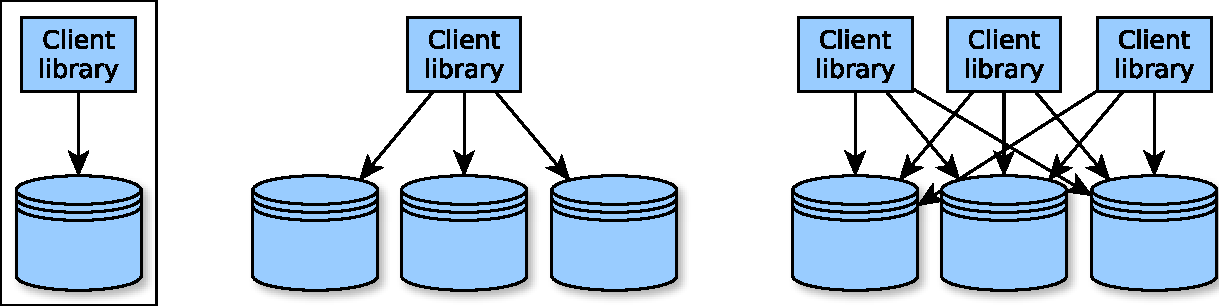
\includegraphics[width=0.9\textwidth]{library-deployment}
    \caption{Use-case scenarios for a sharded CRDT set}
    \label{fig:library_deployment}
  \end{minipage}
\end{figure}

Finally, the flexibility of CRDTs allows to select different synchronization
topologies. One example would be a hierarchical representation where one could
aggregate data in the replica leaves and then propagate updates towards the root
replica, as needed. Another example would be to eventually distribute all
updates in the system according to any gossip or anti-entropy
protocols~\cite{Demers:1987:EAR:41840.41841, Petersen:1997:FUP:268998.266711}. A
combination of these two examples is given in Figure~\ref{fig:sync_topology}.
Here each data center aggregates and internally merges event statistics in a
tree-like manner, while the distribution of updates across all data centers is
done over a mesh topology using an anti-entropy protocol. As shown next in this
chapter, stores and data centers can operate during network partitioning. Many
other use cases can be envisioned since synchronization of CRDTs is highly
customizable: one can decide for each replica in part when and where to pull
updates from.

\begin{figure}[t]
  \centering
  \begin{minipage}{\linewidth}
    \centering
    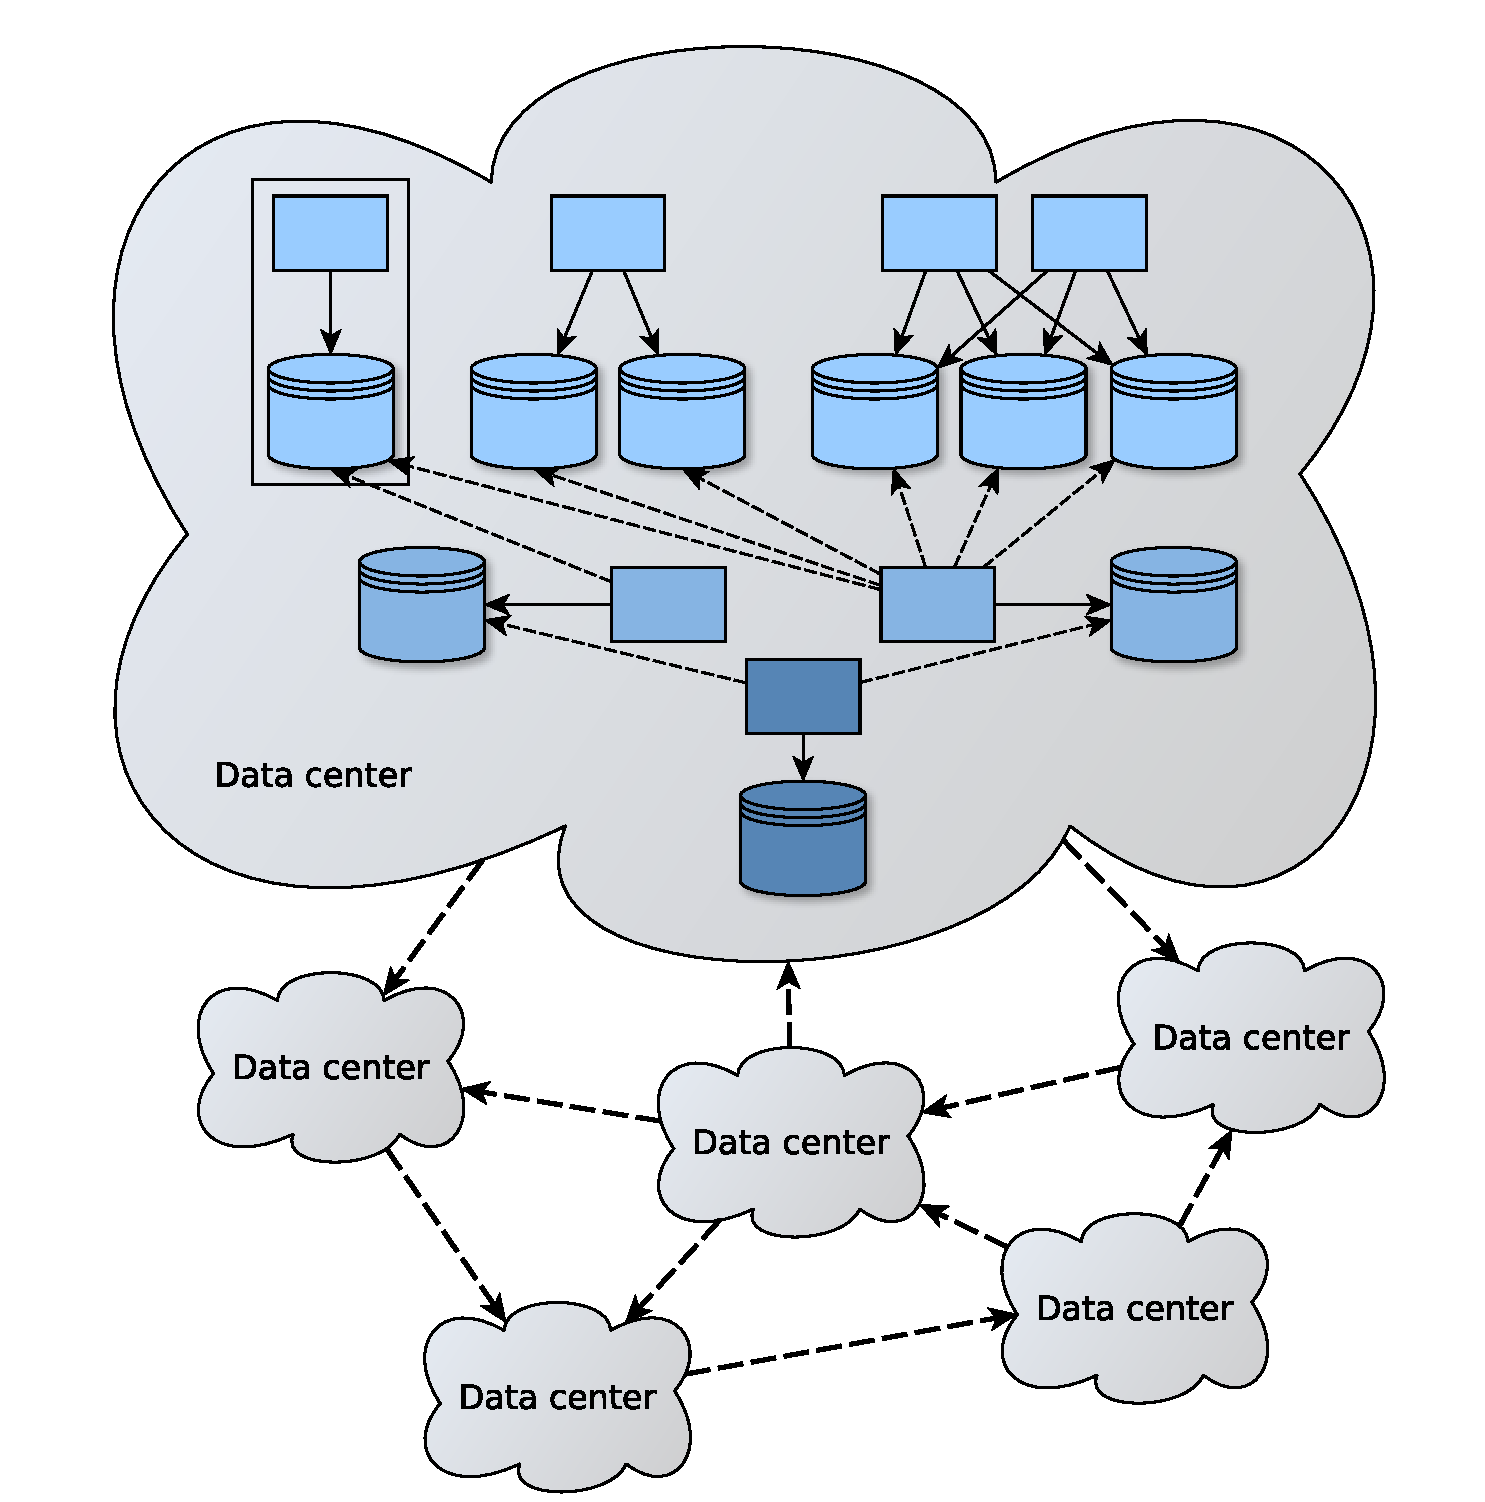
\includegraphics[width=0.7\textwidth]{sync-topology}
    \caption{Example of synchronization topology}
    \label{fig:sync_topology}
  \end{minipage}
\end{figure}


\section{A Delta-based Synchronization Algorithm}
\label{sec:delta-based_synchronization_algorithm}

\begin{algorithm}[t]
\small{
	\floatname{algorithm}{Specification}
	\caption{OR-Set with delta-based synchronization (state-based)}
 	\label{alg:or_set_with_deltas}                       

 	\begin{algorithmic}[1]
 	  \State \Payload $A = \varnothing, R = \varnothing, T = [\,]$
 	  
 	  \State \Query $lookup(e) : \text{boolean}$
 	  \State \hspace{\algorithmicindent} \Return $\exists (e, t, r) \in A \land \nexists (e, t, r, t', r') \in R$
 	  
 	  \State \Update $add(e)$
 	  \State \hspace{\algorithmicindent} \Let $r = replica()$
 	  \State \hspace{\algorithmicindent} \Let $t = T[r] + 1$
 	  \State \hspace{\algorithmicindent} $A \coloneqq A \cup \{(e, t, r)\}$
 	  \State \hspace{\algorithmicindent} $T[r] \coloneqq  t$

 	  \State \Update $remove(e)$
 	  \State \hspace{\algorithmicindent} \Pre $lookup(e)$
 	  \State \hspace{\algorithmicindent} \Let $r' = replica()$
 	  \State \hspace{\algorithmicindent} \Let $t' = T[r'] + 1$
 	  \State \hspace{\algorithmicindent} $R \coloneqq R \cup \{(e, t, r, t', r') \mid \exists (e, t, r) \in A\}$
 	  \State \hspace{\algorithmicindent} $T[r'] \coloneqq  t'$

 	  \State \Compare $(S_{1}, S_{2}) : \text{boolean}$
 	  \State \hspace{\algorithmicindent} \Return $S_{1}.A \subseteq S_{2}.A \land S_{1}.R \subseteq S_{2}.R \land S_{1}.T[i] \leq S_{2}.T[i], \forall i$

 	  \State \Merge $(S_{1}, S_{2}) : \text{payload}$
 	  \State \hspace{\algorithmicindent} \Let $A' = \{(e, t, r) \in S_{2}.A \mid S_{1}.T[r] < t\}$
 	  \State \hspace{\algorithmicindent} \Let $R' = \{(e, t, r, t', r') \in S_{2}.R \mid S_{1}.T[r'] < t'\}$
 	  \State \hspace{\algorithmicindent} \Let $P.A = S_{1}.A \cup A'$
 	  \State \hspace{\algorithmicindent} \Let $P.R = S_{1}.R \cup R'$
 	  \State \hspace{\algorithmicindent} \Let $P.T = max(S_{1}.T, S_{2}.T)$
 	  \State \hspace{\algorithmicindent} \Return $P$
	\end{algorithmic}
 }
\end{algorithm}

A design for a state-based OR-Set which employs a delta-based algorithm
for merging replica states is given in
Specification~\ref{alg:or_set_with_deltas}. In addition to the original
state-based OR-Set which had sets $A$ and $R$ for added and, respectively,
removed elements, the payload now has also a \textit{timestamp vector} $T$ which
has as many components as there are replicas and for which $T[r]$ records the
latest known version of replica $r$. For this purpose, it is assumed that each
replica has a unique identifier that can be retrieved through the function
\textit{replica} and that $T$ can be indexed with this identifier. For example,
if there are $N$ replicas, the \textit{replica} function can simply generate a
number in the range $[0,\ldots,N-1]$ and $T$ can be an integer array of size
$N$. Alternatively, \textit{replica} can generate a string identifying the
replica and $T$ in this case will be a hash table with string keys and integer
values.

Adding a new element $e$ at replica $r$ increments the corresponding component
$T[r]$ to obtain $t$ and inserts the tuple $(e, t, r)$ into set $A$. Compared to
the basic OR-Set, the change was essentially to split the tag which uniquely
identified each element into the pair $(t, r)$. In this way, the elements still
remain tagged, but now we also have the information about the partial order of
updates occurring at each replica, i.e. we know that tuple $(e, t, r)$ was added
before tuple $(e', t', r)$ at replica $r$ if $t < t'$. Removing an element uses
the same principle. Being an OR-Set data type, only locally observed elements at
the source are removed. The logical clock corresponding to the replica is
increased again to keep track of this update. Looking up an element $e$ in the
set translates to verifying if there is an added tuple containing $e$ and
does not exist a corresponding remove tuple.

Remember that the \textit{merge} method in the traditional OR-Set computed the
union between the $A$s and between the $R$s. For any two sets $X$ and $Y$, it is
known that the following holds: $X \cup Y = X \cup (Y \setminus X)$. Since the
goal is to transfer only the difference between sets from one replica to the
other and not the whole set, the right-hand side formula is used. This is done
with the help of timestamp vector $T$. To exemplify, let us consider that we
want to merge the state of Replica~2 into Replica~1. In the first step,
Replica~1 sends its $T$ to Replica~2. Replica~2 then computes the updates based
on this vector: missing tuples are those added or removed at Replica~2 which are
not present in Replica~1, i.e. the logical clock is less than the tuple's
timestamp: $A' = \{(e, t, r) \in S_{2}.A \mid S_{1}.T[r] < t\}$. This set of
updates together with Replica~2's timestamp vector are sent back to Replica~1.
Finally, Replica~1 inserts the updates in the corresponding sets and then
updates its timestamp vector with the maximum between the current one and the
received one component-wise: $P.T = max(S_{1}.T, S_{2}.T)$. This last operation
is required so that the next \textit{merge} will only ask for the updates after
this time.

Thus, the timestamp vector helps to compute the difference between two sets by
filtering based on the tuples timestamp. In this sense, it acts as a vector
clock~\cite{mattern1988virtual} which guarantees the partial order between
updates. Also, because of the transitivity property of the vector clock, each
$\textit{merge}(S_{1}, S_{2})$ includes not only the updates originated at
$S_{2}$ but also those from $S_{3}$ which were pulled by $S_{2}$ but not by
$S_{1}$.

Figure~\ref{fig:or_set_with_delta} shows how the states evolve in this new
OR-Set when applying the same operations as in the previous example from
Figure~\ref{fig:or_set_op_based}.

\begin{figure}[t]
  \centering
  \begin{minipage}{\linewidth}
    \centering
    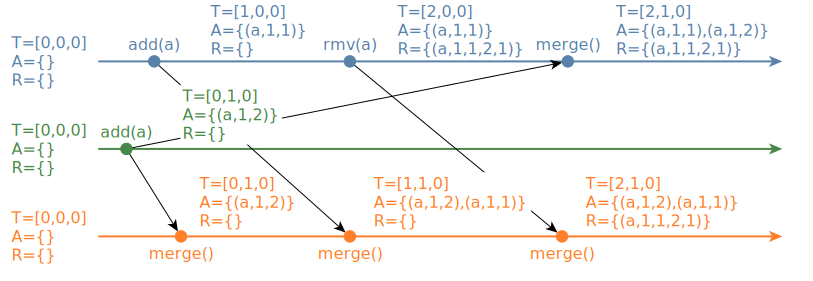
\includegraphics[width=1\textwidth]{or-set-with-delta}
    \caption{OR-Set with delta-based synchronization (state-based)}
    \label{fig:or_set_with_delta}
  \end{minipage}
\end{figure}

\begin{proof}[Proof that delta-based synchronization maintains the CRDT
properties] 
In order to prove that this construct is a CRDT, consider the
partial order $(S, \sqsubseteq)$, where $\sqsubseteq$ is given by the
\textit{compare} method in the specification. Both \textit{add} and
\textit{remove} methods add elements to the payload and increment $T$ and
therefore advance the state in the partial order. Furthermore, it was shown
above that \textit{merge} basically computes the union of the added and,
respectively, removed sets and the maximum of the two timestamp vectors. Hence
we have $\textit{merge}(S_{1}, S_{2}) = S_{1} \sqcup S_{2}$ (LUB) which
concludes the proof.
\end{proof}

\section{Sharding}
\label{sec:sharding}

The next improvement to the OR-Set is partitioning, or sharding, a replica into
many disjunctive subsets which can be stored individually on different machines.
Therefore, each replicated set can reside in a cluster, as illustrated in
Figure~\ref{fig:sharding_meaning}. Here Replica~1 is sharded in 3 subsets,
Replica~2 is sharded in 2 subsets, while Replica~3 is stored entirely on one
machine. This OR-Set data type where each replica set is sharded into subsets
will be referred to as \textbf{Sharded OR-Set} (\textbf{SOR-Set}).

\begin{figure}[b]
  \centering
  \begin{minipage}{1\linewidth}
    \centering
    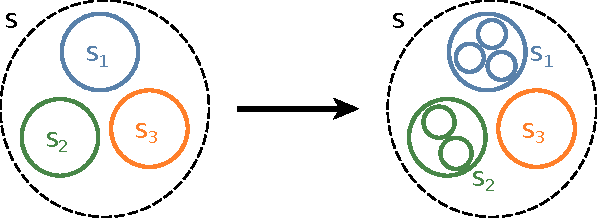
\includegraphics[width=0.45\textwidth]{sharding-meaning}
    \caption{Sharding of OR-Sets}
    \label{fig:sharding_meaning}
  \end{minipage}
\end{figure}

In order to coordinate incoming requests for each of the replicated set, a
client entity is used which forwards the usual $\textit{add}(e)$,
$\textit{remove}(e)$, and $\textit{lookup}(e)$ operations to the corresponding
subset. For this purpose, the client can employ any partitioning function, such
as a hash function with uniform distribution, which maps each element $e$ to a
shard. The client is also responsible for initiating the \textit{merge}
operation between two clusters to pull the updates from all shards in the remote
cluster and distribute them according to the same hash function to the shards in
the local cluster. It does not matter where the client resides as long as it
knows how to communicate with both clusters. For example, one way is for the
client to know the topology and to talk to each shard. Another way would be to
use a DHT overlay for each cluster which the client can bootstrap onto. Then the
client request would bounce in the overlay network until it reaches the shard
which is responsible for that element. For further details about the
architecture, the reader is referred to Section~\ref{sec:architecture}.

\begin{algorithm}[h!]
\small{
	\floatname{algorithm}{Specification}
	\caption{SOR-Set with delta-based synchronization (state-based)}
 	\label{alg:sor_set}                       

 	\begin{algorithmic}[1]
      \State \Payload $A_{i}^{j} = \varnothing, R_{i}^{j} = \varnothing, T_{i}^{j} = [\,][\,], \forall j \in \{1,\ldots,|rc_{i}|\}$
      \State \textcolor{gray}{\Comment{$rc_{i}$ - Replica cluster $i$; $rs_{i}^{j}$ - Replica shard $j$ of $rc_{i}$}}

 	  \State \Query $lookup_{i}(e) : \text{boolean}$
 	  \State \hspace{\algorithmicindent} \Let $j = hash_{i}(e)$
 	  \State \hspace{\algorithmicindent} \Return $\exists (e, t, rc, rs) \in A_{i}^{j} \land \nexists (e, t, rc, rs, t', rc', rs') \in R_{i}^{j}$

 	  \State \Update $add_{i}(e)$
 	  \State \hspace{\algorithmicindent} \Let $j = hash_{i}(e)$
 	  \State \hspace{\algorithmicindent} \Let $rc = rc_{i}$
 	  \State \hspace{\algorithmicindent} \Let $rs = rs_{i}^{j}$
 	  \State \hspace{\algorithmicindent} \Let $t = T_{i}^{j}[rc][rs] + 1$
 	  \State \hspace{\algorithmicindent} $A_{i}^{j} \coloneqq A_{i}^{j} \cup \{(e, t, rc, rs)\}$
 	  \State \hspace{\algorithmicindent} $T_{i}^{j}[rc][rs] \coloneqq t$

 	  \State \Update $remove_{i}(e)$
 	  \State \hspace{\algorithmicindent} \Pre $lookup_{i}(e)$
 	  \State \hspace{\algorithmicindent} \Let $j = hash_{i}(e)$
 	  \State \hspace{\algorithmicindent} \Let $rc' = rc_{i}$
 	  \State \hspace{\algorithmicindent} \Let $rs' = rs_{i}^{j}$
 	  \State \hspace{\algorithmicindent} \Let $t' = T_{i}^{j}[rc'][rs'] + 1$
 	  \State \hspace{\algorithmicindent} $R_{i}^{j} \coloneqq R_{i}^{j} \cup \{(e, t, rc, rs, t', rc', rs') \mid \exists (e, t, rc, rs) \in A_{i}^{j}\}$
 	  \State \hspace{\algorithmicindent} $T_{i}^{j}[rc'][rs'] \coloneqq t'$
 	  
 	  \State \Compare $(rc_{x}, rc_{y}) : \text{boolean}$
 	  \State \hspace{\algorithmicindent} \Let $\tilde{T}_{x} = version(rc_{x})$
 	  \State \hspace{\algorithmicindent} \Let $\tilde{T}_{y} = version(rc_{y})$
 	  \State \hspace{\algorithmicindent} \Return $(\bigcup_{j} A_{x}^{j} \subseteq \bigcup_{k} A_{y}^{k}) \land (\bigcup_{j} R_{x}^{j} \subseteq \bigcup_{k} R_{y}^{k}) \land (\tilde{T}_{x} \leq \tilde{T}_{y})$
 	  \State \hfill $\forall j \in \{1,\ldots,|rc_{x}|\}; \forall k \in \{1,\ldots,|rc_{y}|\}$
 	  
 	  \State \Merge $(rc_{x}, rc_{y}) : \text{payload}$
 	  \State \hspace{\algorithmicindent} \Let $\tilde{T}_{x} = version(rc_{x})$
 	  \State \hspace{\algorithmicindent} \Let $\tilde{T}_{y} = version(rc_{y})$
      \State \hspace{\algorithmicindent} $\forall j \in \{1,\ldots,|rc_{y}|\}$
      \State \hspace{\algorithmicindent} \hspace{\algorithmicindent} \Let $A' = \{(e, t, rc, rs) \in A_{y}^{j} \mid \tilde{T}_{x}[rc][rs] < t\}$
      \State \hspace{\algorithmicindent} \hspace{\algorithmicindent} \Let $R' = \{(e, t, rc, rs, t', rc', rs') \in R_{y}^{j} \mid \tilde{T}_{x}[rc'][rs'] < t'\}$
      \State \hspace{\algorithmicindent} $\forall j \in \{1,\ldots,|rc_{x}|\}$
      \State \hspace{\algorithmicindent} \hspace{\algorithmicindent} \Let $Z.A_{x}^{j} = A_{x}^{j} \cup \{(e, t, rc, rs) \in A' \mid j = hash_{x}(e)\}$
      \State \hspace{\algorithmicindent} \hspace{\algorithmicindent} \Let $Z.R_{x}^{j} = R_{x}^{j} \cup \{(e, t, rc, rs, t', rc', rs') \in R' \mid j = hash_{x}(e)\}$
      \State \hspace{\algorithmicindent} \hspace{\algorithmicindent} \Let $Z.T_{x}^{j} = max(T_{x}^{j}, \tilde{T}_{y})$
      \State \hspace{\algorithmicindent} \Return $Z$
	\end{algorithmic}
 }
\end{algorithm}

Specification~\ref{alg:sor_set} synthesizes the usual state-based operations.
Each replica $i$ of the set is stored in a \textit{replica cluster} $rc_{i}$.
Inside the cluster $rc_{i}$, the set is partitioned into $|rc_{i}|$ subsets,
called \textit{replica shard}s $rs_{i}^{j}$. Therefore, any shard is uniquely
identified by the pair of identifiers $(rc, rs)$. Based on this observation,
instead of using a timestamp vector to keep track of the latest versions for the
replicas as in the previous section, a \textit{timestamp ``matrix''} $T$ is
used. This is actually a degenerated matrix which has as many rows as there are
clusters and which on row $rc_{i}$ has $|rc_{i}|$ columns. Similar to the OR-Set
with delta-based synchronization, each cell $T[rc][rs]$ stores the latest
version of the logical clock of the shard $(rc, rs)$. Each shard has its own $T$
matrix. Since when adding or removing an element from the source replica, it
will be added or, respectively, removed from only one shard $(rc, rs)$ (the one
computed by the hash function), each update can be uniquely tagged with the
tuple $(t, rc, rs)$, where $t$ is the timestamp generated at $(rc, rs)$.

Returning to the specification, the payload is also distributed: $A_{i}^{j}$,
$R_{i}^{j}$, and $T_{i}^{j}$ are, respectively, the set of added and removed
elements and the timestamp matrix for shard $rs_{i}^{j}$. Adding an element
$e$ at replica source $i$ has to first determine in which shard it should be
stored by calling $hash_{i}(e)$. Each cluster may have its own distinct
partitioning function. The procedure then increments the logical clock of that
shard and inserts the tuple $(e, t, rc_{i}, rs_{i}^{j})$ into the set of added
elements $A_{i}^{j}$. Removing an element $e$ follows the same principle as
before: locally observed elements $e$ are tagged and added to the remove set
$R_{i}^{j}$. An element will be in the set if it is in $A_{i}^{j}$ and not in
$R_{i}^{j}$.

Merging the state of a remote replica from cluster $rc_{y}$ into the local state
in cluster $rc_{x}$ proceeds as follows. First, it computes $\tilde{T}_{x} =
version(rc_{x})$ using the formula:
\begin{eqnarray*}
\tilde{T}_{x}[rc][rs] = \begin{cases}
                            max (\bigcup_{j \in \{1,\ldots,|rc_{x}|\}} T_{x}^{j}[rc][rs]) &, \text{if } rc = rc_{x} \\
                            min (\bigcup_{j \in \{1,\ldots,|rc_{x}|\}} T_{x}^{j}[rc][rs]) &, \text{otherwise }
                          \end{cases}
\\
\hfill \forall rc = rc_{i}, i \in \{1,\ldots,N\}; \forall rs = rs_{i}^{j}, j \in \{1,\ldots,|rc_{i}|\}
\end{eqnarray*}

What the \textit{version} function does is to determine a minimum version for
the whole cluster by combining the information from all timestamp matrices $T$.
This is needed because clusters may have different sizes and thus $T_{x}^{j}$
does not necessarily have a correspondent $T_{y}^{j}$. The version is basically
computed by choosing the minimum from all $T_{x}^{j}$ component-wise, except for
the row $rc_{x}$, where the maximum is chosen instead. Updating the set $i$
changes only row $rc_{i}$ in all $T_{i}^{j}$ since each shard increments its own
counter only. Therefore, after $m$ updates to shard $rs_{i}^{j}$, assuming no
synchronization takes place, $T_{i}^{j}[rc_{i}][rs_{i}^{j}] = m$ and
$T_{i}^{j}[rc_{i}][rs_{i}^{k}] = 0, \forall k \ne j$, while the rest of the
cells remain unaffected. For this reason, on row $rc_{x}$ of $\tilde{T}_{x}$,
the maximum value has to be chosen. The procedure is identical for remote
cluster $rc_{y}$.

The next step in the delta-based synchronization algorithm is to compute the
updates in $rc_{y}$ which are missing in $rc_{x}$. For this, $\tilde{T}_{x}$
is used to apply the same principle as before: missing updates are those whose
timestamp is greater than the corresponding logical clock of the local cluster.
Sets $A'$ and $R'$ gather all these updates from all shards in the remote
cluster $rc_{y}$. What remains is to distribute them in $rc_{x}$ according to
the $hash_{x}$ function and to update the timestamp matrix of all shards
$rs_{x}^{j}$.

Lastly, some important observations should be made regarding the SOR-Set. First,
it is still an OR-Set at the core, which means it has the same semantics:
$\textit{add}(e)$ operation has precedence when $\textit{add}(e) \parallel
\textit{remove}(e)$ and $\textit{remove}(e)$ removes locally observed elements
$e$. Second, it employs the delta-based synchronization algorithm introduced in
Section~\ref{sec:delta-based_synchronization_algorithm}. Third, the
\textit{merge} operation remains unobtrusive like for all CRDTs: clients can
issue requests to the set while the operation progresses in the background.
Since the minimum version matrix $\tilde{T}_{y}$ is computed first, the remote
cluster $rc_{y}$ can meanwhile process any subsequent updates. They will be
pulled with the next merge. Analogously, because at the end each $T_{x}^{j}$ is
updated to the maximum between the current one and the remote one
component-wise, the local cluster can in this time process any incoming client
requests. Therefore, both sets can be updated while the synchronization takes
place. The last observation to make is that this algorithm is resilient to shard
failures in both local and remote clusters. An unreachable shard in the local
cluster leads to a potential bigger $\tilde{T}_{x}$ except for row $rc_{x}$.
This means that not all updates will be fetched. As soon as the failed shard
restores, its lagging timestamp will lead to a smaller $\tilde{T}_{x}$ and the
next merge will thus include the missing updates plus some of the already
fetched ones. For the remote cluster, an unreachable shard has the same
consequence: $T_{x}^{j} \coloneqq max(T_{x}^{j}, \tilde{T}_{y})$ will set
smaller values in row $rc_{y}$ and missed updates will be fetched with the next
merge after the shard restores. These failure scenarios are tested and discussed
in Section~\ref{sec:unit_tests}.

\begin{proof}[Proof that sharding maintains the CRDT properties]
Consider a replica state as $s_{i} = (A_{i}, R_{i}, \tilde{T}_{i})$, where
$A_{i} = \bigcup_{j \in \{1,\ldots,|rc_{i}|\}} A_{i}^{j}$, $R_{i} = \bigcup_{j
\in \{1,\ldots,|rc_{i}|\}} R_{i}^{j}$, and $\tilde{T}_{i}$ was defined above.
Thus, a set is characterized by the contributions of all its subsets. The
partial order is then $(S, \sqsubseteq)$, $\forall s_{i} \in S$ and
$\sqsubseteq$ given by \textit{compare} method. Update operations \textit{add}
and \textit{remove} advance the state in the partial order as they both add
elements to the set and increase $\tilde{T}$. \textit{Merge} computes the set
union between $A_{x}$ and $A_{y}$ and between $R_{x}$ and $R_{y}$, respectively.
Also, because each $T_{x}^{j}$ is updated with the maximum between $T_{x}^{j}$
and $\tilde{T}_{y}$, the newly obtained $\tilde{T}_{x}$ will be the maximum
between $\tilde{T}_{x}$ and $\tilde{T}_{y}$. Therefore \textit{merge} computes
the LUB, which concludes the proof.
\end{proof}

\section{Garbage Collection}
\label{sec:garbage_collection}

As seen in Specification~\ref{alg:sor_set}, update procedures add tuples to
either $A$ or $R$ sets, which lead to an increase of database in size. If we
want to always have a complete history for a replica, then the behavior may
conform to these requirements. However, due to space constraints, this
assumption is usually not practical. Hence, this section introduces an automatic
garbage collection mechanism for removing, or \textit{expiring}, tuples from
these sets after a specified time interval. To this extent, elements are
considered to have limited lifetime in the store, setting that can be configured
based on application semantics. For example, we may not be interested in IP
addresses for logging into a given user account which are older than one month.

Any $(e, t, rc, rs) \in A$ from the SOR-Set specification will be referred to as
an \textit{ADD(e)} tuple and any $(e, t, rc, rs, t', rc', rs') \in R$ as an
\textit{RMV(e)} tuple. These tuples are generated either when the client calls
\textit{add} and \textit{remove} methods, or through the synchronization
process. Lookup semantics states that $\textit{lookup}(e)$ should return
\textit{true} if $e$ is in the SOR-Set and \textit{false} otherwise. The
following theorem on tuple expiration can now be formulated.

\begin{theorem}[\textbf{Tuple expiration}]
\begin{itshape}
If, at any given shard, the tuples corresponding to any element $e$,
\textit{ADD(e)} and \textit{RMV(e)}, are expired in the same order in which they
were originally inserted, then the lookup semantics are preserved.
\end{itshape}
\end{theorem}

\begin{proof}
Let us first consider update operations occurring at one replica with no
synchronization taking place. There are two cases: i) $ADD(e) \rightarrow
RMV(e)$, meaning \textit{ADD(e)} is inserted before \textit{RMV(e)}. The
expected return value for $\textit{lookup}(e)$ after these operations are
executed is evidently \textit{false}. If \textit{ADD(e)} expires first and
\textit{RMV(e)} expires later, then the semantics does not change. If, however,
expiration occurs in reverse order, there will be a time window when
\textit{ADD(e)} is present, but \textit{RMV(e)} not. In this interval, a
$\textit{lookup}(e)$ call will return \textit{true}, which will change the
expected semantics. ii) $RMV(e) \rightarrow ADD(e)$. The proof follows the same
rationale.

Consider now the situation when tuples propagate from one shard to another.
Again there are two cases: i) $ADD(e) \leadsto RMV(e)$, which symbolizes that
\textit{ADD(e)} was originally inserted at one shard, fetched through replica
synchronization and then a \textit{RMV(e)} was inserted locally. As soon as the
remote \textit{ADD(e)} is inserted in the local set, this case reduces to the
corresponding sequential one from before: $ADD(e) \rightarrow RMV(e)$ and both
tuples should be expired in the same order in which were originally inserted.
If the \textit{RMV(e)} is inserted before \textit{ADD(e)} reaches the local
shard, these updates are concurrent and $ADD(e)$ wins: $\textit{lookup}(e)$ will
return \textit{true} as long as the $ADD(e)$ is not expired, which is what we
expect. ii) $RMV(e) \leadsto ADD(e)$. Similarly, the case reduces to the
sequential $RMV(e) \rightarrow ADD(e)$.
\end{proof}

The following changes could be made to the SOR-Set specification in order to
include an automatic garbage collection while maintaining the lookup semantics. 
\textit{Garbage} which can be reclaimed refers to all the expired tuples in the
store. The idea is to associate a \textit{time-to-live} (TTL) value with each
tuple when it is inserted into the corresponding set through an \textit{add} or
\textit{remove}. This value represents the time interval from the moment it was
inserted after which the tuple will expire and can be expressed in any time
unit, e.g. minutes, hours, days, etc. In this way, tuples older than a specified
period are considered to be no longer relevant and can be safely discarded. Data
stores such as Redis~\cite{redis} or Cassandra~\cite{cassandra} offer support
for setting TTL attributes to records and automatic removal for expired ones.
Otherwise, a simple periodic scan-and-remove process on the database can be
used.

Thus, set $A$ will contain pairs $\langle(e, t, rc, rs), TTL(e)\rangle$ and set
$R$ will contain pairs $\langle(e, t, rc, rs, t', rc', rs'), TTL(e)\rangle$. To
ensure that tuples corresponding to $e$ expire in the order in which they were
added, it is sufficient to stamp them with the same value $TTL(e)$. This initial
value will gradually decrease until it reaches 0 and then the tuple can be
removed. When copying the tuples to other shards, their remaining TTL is
preserved, i.e. the current TTL at the remote replica is transferred together
with the tuple to the local replica. By doing this, tuples will expire at the
local replica in the same order as they do at the remote one.

Because it is possible for $ADD(e)$ to be added on a shard, copied to another
shard, and then here a $RMV(e)$ inserted, all replicas are required to use the
same $TTL(e)$ function for stamping tuples of a particular element $e$. However,
it is not a requirement for having the same physical clock speed on all machines
or for having their clocks periodically synchronized. What is needed is only a
partial order on the tuples expiration as stated by the above theorem.
Preserving the TTLs for tuples when propagating them across different shards
evidently does not imply that there is a global time point when all copies of
one tuple are expired simultaneously. In fact, copies of the tuples in local
cluster will expire shortly after the original ones in remote cluster have
expired. This happens because time freezes for copies while they are in transit
and their TTLs remain constant. However, this does not invalidate the lookup
semantics according to the tuple expiration theorem.

\begin{proof}[Proof that garbage collection maintains the CRDT properties]
In order to prove that this SOR-Set construct together with the garbage
collection mechanism described above retains the CRDT properties, we consider
first the case when no sharding is used. A new partial order can be defined by
the relation $S_{1} \sqsubseteq S_{2} \iff S_{1} \subseteq S_{2} \lor S_{1}
\equiv (S_{1} \cap S_{2})$. The first term holds when no tuples are expired and
thus either \textit{add} or \textit{remove} operation increases the
corresponding set like before. If by the time we apply any operation, some
tuples are expired from $S_{1}$, then the states containing old non-expired
tuples from before and after the update are considered equivalent, i.e. any
$\textit{lookup}(e)$ method on either $S_{1}$ or $S_{1} \cap S_{2}$ returns the
same result. It is easy to see that, relative to $\sqsubseteq$, the updates
always advance the states in the partial order. Taking sharding into account, we
can simply consider the union of all $A$ and, respectively, $R$ sets in one
cluster as in Specification~\ref{alg:sor_set}: $S_{i} = \bigcup_{\forall j \in
\{1,\ldots,|rc_{i}|\}} S_{i}^{j}$, where $S$ is $A$ or $R$. From this point, the
proof follows the same rationale as for the SOR-Set.
\end{proof}
